\documentclass{beamer}

% packages
\usepackage{graphicx,amsmath,amsfonts,amssymb,listings,tikz,multimedia}

% themes & colors
\usetheme{Copenhagen}
\usecolortheme{beaver}
\beamerdefaultoverlayspecification{<+->}

% user commands
\newcommand{\weeknum}{0}

\begin{document}

  \section{Group Meeting}
  \title{Group Meeting}
  \author{Brandon Gusto}

  \institute{Dept. of Scientific Computing \\ Florida State University}
  \date{\today}
  \frame{\titlepage}

  \begin{frame}{Highlights}
    \begin{block}{Highlights }
      \begin{itemize}
        \setlength\itemsep{1em}
        \item Identified Multiresolution/AMR issue: multiresolution-based prolongation routine
            caused artifacts
        \item Multiresolution scheme works well in parallel, as long as buffer region is not added
      \end{itemize}
    \end{block}
  \end{frame}

  \begin{frame}
    \begin{figure}
      \center
      \movie[width=0.5\textwidth,height=0.4\textwidth, poster]{}{movie.avi}
    \end{figure}
  \end{frame}

  \begin{frame}{Buffer Region Filling}
    \begin{figure}
      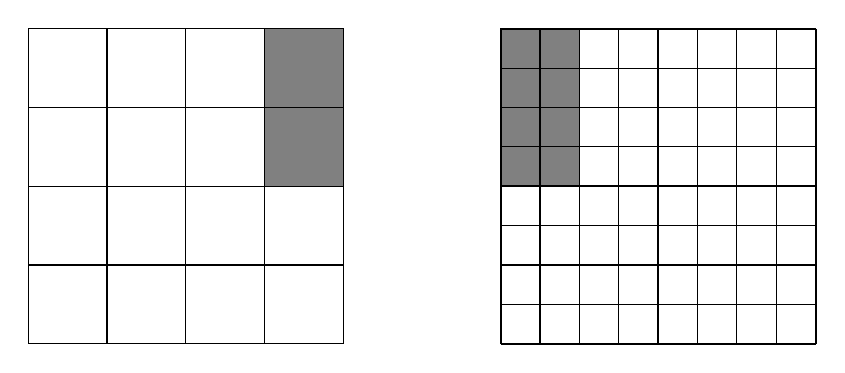
\begin{tikzpicture}

  % draw grids
  \draw [fill=gray] (0,2) rectangle (1,4);
  \draw [fill=gray] (-3,2) rectangle (-2,4);
  \draw [step=0.5cm] (0,0) grid (4,4);
  \draw [thick] (0,0) -- (0,4);
  \draw [thick] (0,0) -- (4,0);
  \draw [thick] (0,4) -- (4,4);
  \draw [thick] (4,4) -- (4,0);
  \draw [thick] (2,0) -- (2,4);
  \draw [thick] (0,2) -- (4, 2);
  \draw [step=1.0cm] (-6,0) grid (-2,4);

\end{tikzpicture}

    \end{figure}
  \end{frame}

  \begin{frame}{Task List (TO-BE-COMPLETED)}
    \begin{block}{Tasks}
      \begin{itemize}
        \setlength\itemsep{1em}
        \item Complete mask filling cases for 2D
        \item Parallel communication of mask information to blocks across processors (in 1D and 2D)
      \end{itemize}
    \end{block}
  \end{frame}

\end{document}
